\chapter{Image Formation}
\label{ch:lesson26}

Up to now we have been processing images without thinking about where they come from. This chapter unpacks that mystery by considering: \textbf{geometry} (how the projection matrix is derived from a pinhole camera model), \textbf{optics} (what a real lens does that a pinhole camera fails to model --- focus and blur), and \textbf{sensing/color} (how a real sensor captures only one color per pixel and needs to reconstruct the rest, along with the two classic pitfalls --- gamma and white balance --- that trip up naive image processing).

\section{The pinhole projection matrix, derived}

A pinhole camera only lets through rays of light passing through a particular point (the \emph{center of projection}). By similar triangles, a 3D point $(X,Y,Z)$ (camera-centered coordinates) lands on the image plane at
\begin{equation}
x = f\frac{X}{Z}, \qquad y = f\frac{Y}{Z},
\end{equation}
where $f$ is the distance from the pinhole to the image plane. Converting to pixel units requires the \textbf{intrinsics} $K$; incorporating the camera's position and orientation relative to the world requires the \textbf{extrinsics} $[R|t]$. Put together, in homogeneous coordinates:
\begin{equation}
\underbrace{\begin{bmatrix}u\\v\\1\end{bmatrix}}_{\text{pixel}} \;\propto\; \underbrace{\begin{bmatrix}f_x&0&c_x\\0&f_y&c_y\\0&0&1\end{bmatrix}}_{K}\underbrace{\begin{bmatrix}R & t\end{bmatrix}}_{\text{extrinsics}}\begin{bmatrix}X\\Y\\Z\\1\end{bmatrix}_{\text{world}}.
\end{equation}
This is exactly the $P=K[R|t]$ that Chapters~\ref{ch:lesson27}--\ref{ch:lesson29} (Camera Calibration, Epipolar Geometry, and Structure from Motion) will use. Every symbol traces back to a physical cause: $f_x,f_y$ to focal length and pixel size; $(c_x,c_y)$ to where the optical axis hits the sensor (the \emph{principal point}); $R,t$ to the camera's pose. Figure~\ref{fig:l26-1} shows a cube projected through $P$.

\begin{figure}[h]
\centering
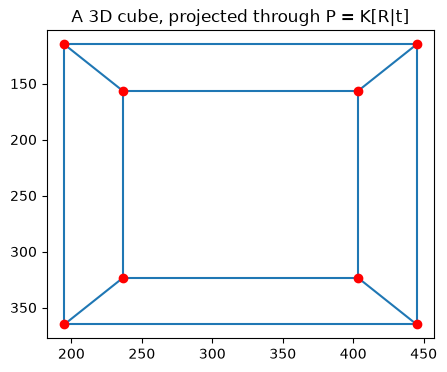
\includegraphics[width=0.4\textwidth]{figures/lesson26_fig01.png}
\caption{A 3D cube, projected through $P=K[R|t]$ onto the image plane.}
\label{fig:l26-1}
\end{figure}

\section{Real lenses: focus and defocus blur}

A pinhole camera lets in so little light that it needs absurdly long exposures. Real cameras use a lens to gather much more light, but lenses focus sharply only for objects at a particular distance (the \textbf{focal plane}). Points nearer or farther than that spread their light over a small disk on the sensor (the \textbf{circle of confusion}) instead of at a point --- exactly the blurring convolution kernels from Chapters~\ref{ch:lesson09}--\ref{ch:lesson10}, just applied with a kernel size that depends on depth. Focusing at $5$m: a near object (depth $2$m) gets kernel size $19$, the object at the focal plane gets kernel size $1$ (unblurred), and a far object (depth $9$m) gets kernel size $25$ (Figure~\ref{fig:l26-2}).

\begin{figure}[h]
\centering
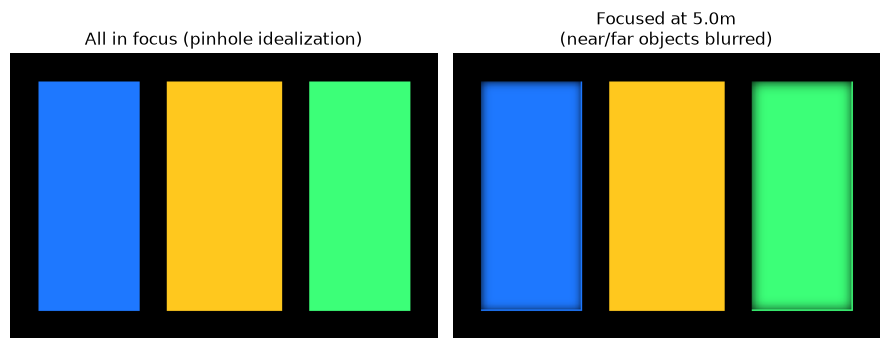
\includegraphics[width=0.85\textwidth]{figures/lesson26_fig02.png}
\caption{All in focus (pinhole idealization) vs.\ focused at $5$m --- near and far objects blur, the mid-depth object stays sharp.}
\label{fig:l26-2}
\end{figure}

This explains why a wider aperture gathers more light (at the expense of a shallower depth of field), while a narrow aperture produces a sharp image (but lets in less light) --- the classic photographic aperture/depth-of-field tradeoff, and the reason portrait photos often blur the background while keeping the subject sharp.

\section{The Bayer color filter array: one color per pixel}

To keep costs down, most camera sensors don't measure red, green, and blue separately at every pixel. Instead, a single monochrome photosensor array sits under a mosaic of tiny color filters, so each individual pixel physically records only \emph{one} of the three colors. The most common arrangement (RGGB) --- the \textbf{Bayer filter} (\citelink{bayer1976}{Bayer, 1976}) --- repeats in a $2\times2$ tile pattern: one red, one blue, and \emph{two} green filters, since the human eye is most sensitive to green. Every pixel in the raw sensor output is therefore missing two-thirds of its color information by construction, as Figure~\ref{fig:l26-3} shows.

\begin{figure}[h]
\centering
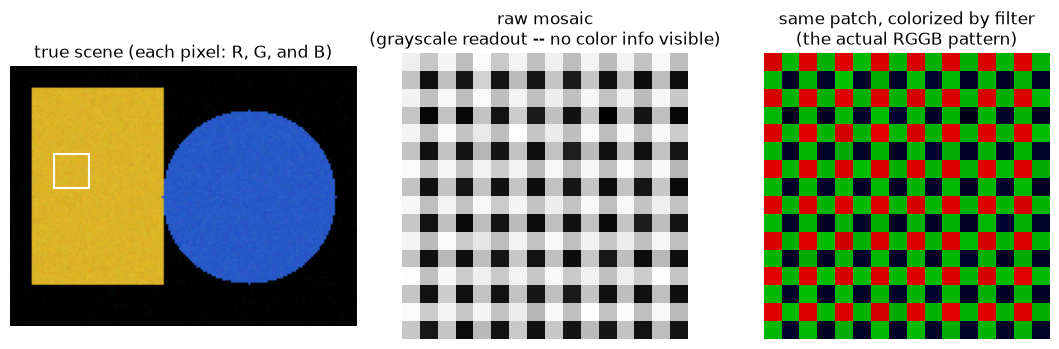
\includegraphics[width=0.95\textwidth]{figures/lesson26_fig03.png}
\caption{A true-color scene, a $16\times16$ crop of the raw Bayer mosaic (grayscale readout, no color visible), and the same crop colorized by filter, revealing the RGGB pattern.}
\label{fig:l26-3}
\end{figure}

\subsection*{Demosaicking: reconstructing RGB from the mosaic}

\textbf{Demosaicking} fills in each pixel's two missing colors by interpolating from same-color neighbors --- the simplest version is bilinear: average the nearby known samples of a color, weighted by distance, exactly Chapter~\ref{ch:lesson09}'s bilinear interpolation, just interpolating across a sparse, patterned grid of known samples. A from-scratch bilinear demosaicker reaches a mean absolute error of $3.37$ against ground truth; \code{cv2.cvtColor(..., cv2.COLOR\_BayerBG2BGR)} reaches $3.43$ --- both land within a fraction of a pixel value of each other, the residual mostly just sensor noise already present in the mosaic (Figure~\ref{fig:l26-4}).

\begin{figure}[h]
\centering
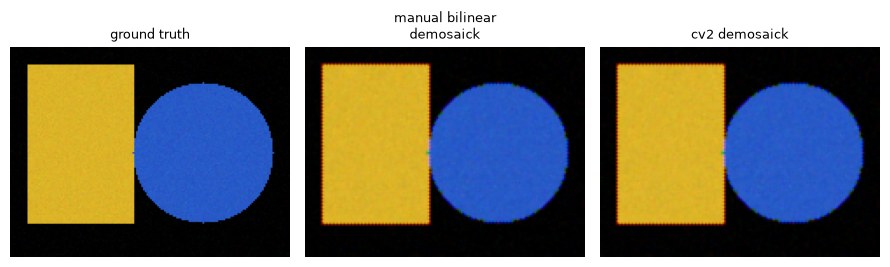
\includegraphics[width=0.9\textwidth]{figures/lesson26_fig04.png}
\caption{Ground truth, manual bilinear demosaick, and \code{cv2} demosaick --- nearly indistinguishable.}
\label{fig:l26-4}
\end{figure}

\subsection*{The pitfall: getting the mosaic pattern wrong}

The R/G/B arrangement matters, and there's more than one convention (RGGB, BGGR, GRBG, GBRG, depending on the sensor). Demosaicking with the \emph{wrong} assumed pattern doesn't fail gracefully --- it silently produces a plausible-looking but badly wrong-colored image, since every pixel gets a value, just the wrong one: the correct pattern gives MAE $3.43$, the wrong pattern jumps to MAE $64.69$ --- nearly a $19\times$ increase, from every red sample being treated as blue and vice versa, as Figure~\ref{fig:l26-5} shows.

\begin{figure}[h]
\centering
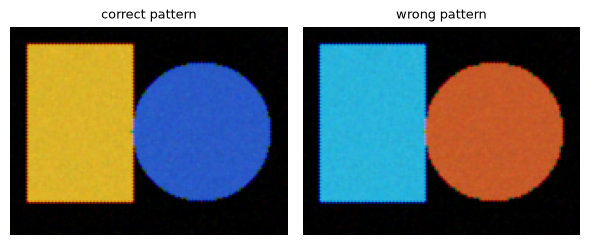
\includegraphics[width=0.6\textwidth]{figures/lesson26_fig05.png}
\caption{Correct vs.\ wrong Bayer pattern assumption --- a strongly color-shifted image.}
\label{fig:l26-5}
\end{figure}

\section{Gamma correction: pixel values are not linear light}

Cameras and displays don't store brightness proportionally to physical light intensity (\textbf{linear radiance}). Instead, values are \textbf{gamma-encoded}: \code{encoded = linear ** (1/gamma)} (typically gamma $\approx 2.2$, close to the sRGB standard), which allocates more encoded levels to darker tones --- matching human vision's greater sensitivity to shadows than highlights. Decoding reverses it: \code{linear = encoded ** gamma}.

\subsection*{The pitfall: averaging encoded pixels is not averaging light}

Blending, resizing, and blurring (Chapters~\ref{ch:lesson08}--\ref{ch:lesson10}) all implicitly assume a linear quantity is being averaged. Pixel values usually aren't linear --- they're gamma-encoded --- so naively averaging two encoded pixel values gives the \emph{wrong physical brightness}. Averaging encoded black and white directly gives $0.500$; the physically correct 50\%-linear-light gray, properly decoded/averaged/re-encoded, is $0.730$ --- the naive result represents only $21.8\%$ of the true linear brightness, not $50\%$, visibly so in Figure~\ref{fig:l26-6}.

\begin{figure}[h]
\centering
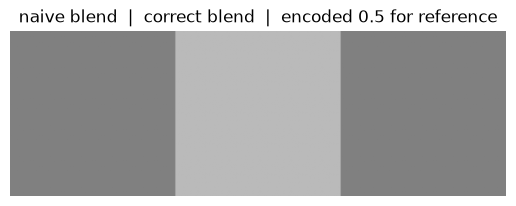
\includegraphics[width=0.55\textwidth]{figures/lesson26_fig07.png}
\caption{Naive blend of encoded black/white (left) vs.\ the physically correct blend (middle) vs.\ encoded $0.5$ for reference (right) --- the naive blend is visibly, dramatically darker.}
\label{fig:l26-6}
\end{figure}

This is a real and common bug when image-processing code (blurring, mipmap generation, alpha blending) operates directly on gamma-encoded pixel values instead of linearizing first.

\section{White balance: color depends on the light source}

A camera records the \emph{product} of a surface's reflectance and the illuminant's color, not the surface's ``true'' color alone --- a white sheet of paper looks orange under warm tungsten light and blue-ish under overcast sky, even though our visual system usually compensates for this automatically (color constancy). Cameras have to do the same correction deliberately: \textbf{white balancing}.

\subsection*{The gray-world assumption}

A simple, classic white-balancing algorithm assumes that, averaged over an entire real-world scene, colors roughly cancel out to neutral gray. Under that assumption, any systematic difference between a photo's per-channel averages reveals the illuminant's color cast, so rescaling each channel to equalize the averages should approximately undo it, as Figure~\ref{fig:l26-7} demonstrates.

\begin{figure}[h]
\centering
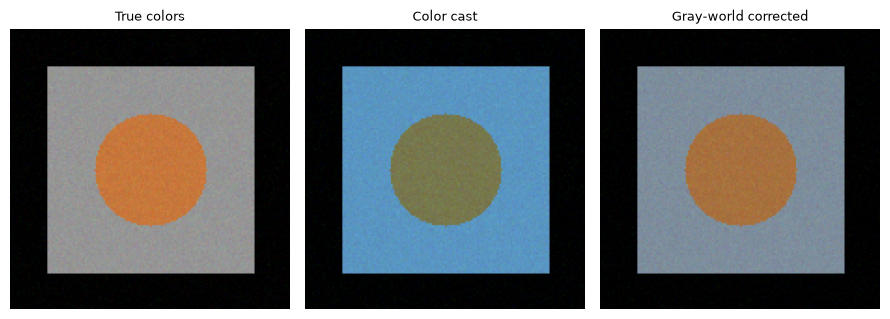
\includegraphics[width=0.9\textwidth]{figures/lesson26_fig09.png}
\caption{True colors, under a warm tungsten cast, and gray-world corrected. Mean absolute pixel error drops from $18.98$ to $7.43$ after correction --- substantial, though not to zero, since this small scene (dominated by a colored circle) isn't perfectly neutral on average.}
\label{fig:l26-7}
\end{figure}

That residual error is exactly why real cameras often combine gray-world with other cues (an actual detected gray/white reference patch, learned scene statistics, or user-specified presets) rather than relying on the assumption alone.

\subsection*{Exercises}
\begin{enumerate}
  \item Change the defocus \code{strength} parameter to make the depth-of-field effect much shallower (larger \code{strength}) or much deeper (smaller \code{strength}). At \code{strength=0}, what should happen, and does the code produce that?
  \item Build and decode a BGGR mosaic instead of RGGB (swap which corner is red vs.\ blue). Find the matching OpenCV code by trying each of \code{cv2.COLOR\_BayerBG2BGR}, \code{cv2.COLOR\_BayerGB2BGR}, \code{cv2.COLOR\_BayerGR2BGR}, \code{cv2.COLOR\_BayerRG2BGR} and checking which one drops the MAE back down to the noise floor --- OpenCV's naming convention for these codes is notoriously easy to get backwards, itself a small demonstration of this chapter's point about silent pattern-mismatch errors.
  \item Repeat the gamma-blending experiment, but blend $0.2$ and $0.8$ (instead of pure black and white) in both the naive and correct ways. Is the discrepancy between them larger or smaller than the black/white case, and why might that make sense given the shape of the gamma curve?
  \item Modify the white-balance demo so the scene is dominated by a large \emph{saturated red} region instead of a neutral gray card (i.e.\ make gray-world's core assumption clearly false). Does gray-world white balancing still improve the result, make no difference, or actively make it worse?
\end{enumerate}

\vfill
\fullcode{lesson26}{lesson26_image_formation}
